% SC4023 --- Chapter 3: AI for Testing (0->100 ground-up)
\chapter{AI for Testing: Generation, Fuzzing, and Oracles}
\label{ch:testing}
\sloppy

\begin{quote}
\emph{``Testing shows the presence, not the absence of bugs.''} --- Edsger Dijkstra. AI does not change that truth, but it can search for presence far faster and in corners humans rarely look.
\end{quote}

\noindent\fbox{\parbox{\dimexpr\linewidth-2\fboxsep-2\fboxrule}{%
\textbf{From zero: no testing background assumed.} We start from a single function and the question ``did it do what I meant?''---what a test is, what an oracle is, and why writing both by hand does not scale. Every idea appears picture-first, then as a definition you can apply.}}
\vspace{0.4em}

\section*{Learning Outcomes}
After this chapter you will be able to:
\begin{enumerate}[label=(L\arabic*)]
    \item define test cases, oracles, and coverage (line, branch, mutation);
    \item explain why the oracle problem limits automated testing;
    \item describe search-based and LLM-based test-generation techniques;
    \item sketch an AI-guided fuzzing loop and its feedback signals;
    \item apply metamorphic and differential oracles to sidestep missing specifications.
\end{enumerate}

% ============================================================
\section{Why Testing Is Hard: Coverage and Oracles}
\label{sec:why-testing-hard}
\paragraph{Intuition.} To test a function you need two things: an \emph{input} to run it on and a way to judge the \emph{output}. The first is easy to invent; the second is where meaning lives. ``Does \texttt{sort([3,1,2])} return \texttt{[1,2,3]}?'' is a useful oracle. ``Does this web handler behave correctly on all edge cases?'' is a question humans struggle to answer completely.

Formally, a \emph{test case} is a triple $(x, y, \text{check})$ where $x$ is input, $y$ is expected output (or property), and \texttt{check} decides pass/fail. The \emph{oracle problem} is that $y$ is often unspecified, expensive to compute, or itself buggy. Without an oracle, execution is just a run---not a test.

\emph{Coverage} measures how much of the program a suite exercises. \emph{Line coverage} is the fraction of executable lines run; \emph{branch coverage} is the fraction of \texttt{if}/\texttt{switch} edges taken. Higher coverage does not imply correctness, but low coverage guarantees untested behaviour.

\begin{figure}[h]\centering
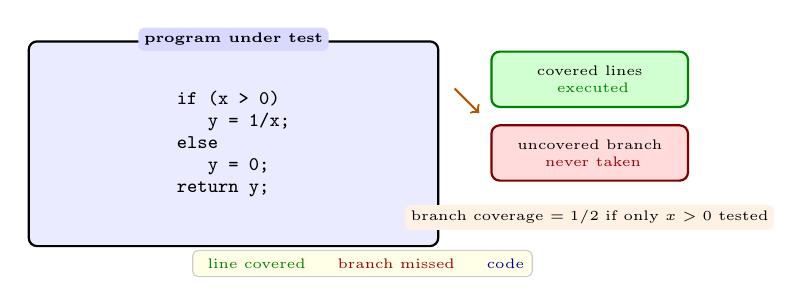
\begin{tikzpicture}[scale=0.78,every node/.style={font=\scriptsize},
  code/.style={draw,thick,rounded corners=3pt,minimum width=5.2cm,minimum height=2.6cm,align=left,inner sep=5pt}]
  \node[code,fill=blue!8] (prog) at (0,0) {\texttt{if (x > 0)}\\\texttt{\ \ \ y = 1/x;}\\\texttt{else}\\\texttt{\ \ \ y = 0;}\\\texttt{return y;}};
  \node[font=\tiny\bfseries,fill=blue!15,rounded corners=2pt,inner sep=2pt] at (0,1.7) {program under test};
  % coverage overlay
  \begin{scope}[xshift=4.2cm]
    \draw[fill=green!18,draw=green!50!black,thick,rounded corners=3pt] (0,0.6) rectangle (3.2,1.5);
    \node[font=\tiny,align=center] at (1.6,1.05) {covered lines\\ \textcolor{green!50!black}{$\blacksquare$ executed}};
    \draw[fill=red!14,draw=red!50!black,thick,rounded corners=3pt] (0,-0.6) rectangle (3.2,0.3);
    \node[font=\tiny,align=center] at (1.6,-0.15) {uncovered branch\\ \textcolor{red!60!black}{$\blacksquare$ never taken}};
    \draw[->,thick,orange!70!black] (-0.6,0.9) -- (-0.2,0.5);
    \node[font=\tiny,fill=orange!10,rounded corners=2pt,inner sep=2pt] at (1.6,-1.2) {branch coverage $=1/2$ if only $x>0$ tested};
  \end{scope}
  \node[font=\tiny,align=left,fill=yellow!10,draw=gray!40,rounded corners=2pt,inner sep=3pt] at (2.1,-1.95) {\textcolor{green!50!black}{$\blacksquare$ line covered} \quad \textcolor{red!60!black}{$\blacksquare$ branch missed} \quad \textcolor{blue!60!black}{$\blacksquare$ code}};
\end{tikzpicture}
\caption{Coverage intuition: running tests lights up lines and branches. Line coverage can be 100\% while branch coverage is 50\%, leaving the \texttt{else} path untested and its bug hidden.}
\label{fig:coverage}
\end{figure}

Two other useful measures: \emph{mutation score} (fraction of seeded artificial faults a suite catches) and \emph{path coverage} (fraction of distinct control-flow paths). Both are stronger but far more expensive.

\begin{definition}[Oracle]
An \emph{oracle} is a procedure $O(x, P(x))$ that returns pass/fail for input $x$ and program output $P(x)$. Examples: a golden output $y^*$ (exact oracle), an assertion $x.\text{length} \ge 0$ (partial oracle), or a relation between two outputs (metamorphic oracle, \S\ref{sec:oracle-problem}).
\end{definition}

% ============================================================
\section{AI-Based Test Generation}
\label{sec:ai-test-gen}
\paragraph{Intuition.} Humans write tests one by one. Machines can propose hundreds, keep those that increase coverage or kill mutants, and discard the rest. The pattern is \emph{generate--execute--filter}: draft candidates, run them, keep what helps.

Two families dominate. \emph{Search-based} tools (e.g., EvoSuite for Java) evolve test suites with a genetic algorithm: fitness is coverage plus mutation kill, mutation adds branches, crossover mixes tests. \emph{LLM-based} tools prompt a code model with the method signature, docstring, and surrounding code and ask it to ``write JUnit tests for \texttt{median}.'' The LLM brings natural-language understanding; search brings systematic coverage.

\begin{figure}[h]\centering
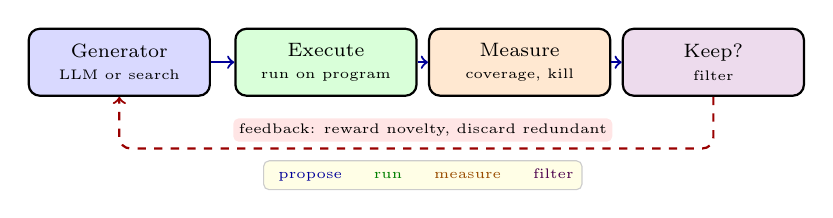
\begin{tikzpicture}[scale=0.82,every node/.style={font=\scriptsize},
  box/.style={draw,thick,rounded corners=4pt,minimum width=2.3cm,minimum height=0.85cm,align=center}]
  \node[box,fill=blue!15] (gen) at (0,0) {Generator\\\tiny LLM or search};
  \node[box,fill=green!15] (exec) at (3.2,0) {Execute\\\tiny run on program};
  \node[box,fill=orange!18] (meas) at (6.2,0) {Measure\\\tiny coverage, kill};
  \node[box,fill=violet!14] (keep) at (9.2,0) {Keep?\\\tiny filter};
  \foreach \a/\b in {gen/exec,exec/meas,meas/keep}
    \draw[->,thick,blue!60!black] (\a) -- (\b);
  \draw[->,thick,red!60!black,dashed,rounded corners=4pt] (keep.south) -- ++(0,-0.8) -- ++(-9.2,0) -- (gen.south);
  \node[font=\tiny,fill=red!10,rounded corners=2pt,inner sep=2pt] at (4.7,-1.05) {feedback: reward novelty, discard redundant};
  \node[font=\tiny,align=left,fill=yellow!10,draw=gray!40,rounded corners=2pt,inner sep=3pt] at (4.7,-1.75) {\textcolor{blue!60!black}{$\blacksquare$ propose} \quad \textcolor{green!50!black}{$\blacksquare$ run} \quad \textcolor{orange!60!black}{$\blacksquare$ measure} \quad \textcolor{violet!60!black}{$\blacksquare$ filter}};
\end{tikzpicture}
\caption{Generate--execute--filter loop. Both EvoSuite and LLM-based generators iterate it; the difference is how candidates are proposed (evolution vs.\ sampling).}
\label{fig:gen-filter-loop}
\end{figure}

\begin{lstlisting}[language=Python, caption={Prompting an LLM to generate tests: give it the function and ask for edge cases.}, label={lst:llm-tests}]
# Function under test
def median(xs):
    if not xs: return None
    s = sorted(xs); n = len(s)
    return s[n//2] if n % 2 == 1 else (s[n//2-1]+s[n//2])/2

# Prompt to LLM (in practice, include file context + docstring):
# "Write pytest tests for median covering empty, odd, even, duplicates, negatives."
def test_median():
    assert median([]) is None          # empty
    assert median([3]) == 3            # single
    assert median([1,2,3]) == 2        # odd
    assert median([1,2,3,4]) == 2.5    # even
    assert median([2,2,2]) == 2        # duplicates
    assert median([-5,-1,0]) == -1     # negatives
# LLM drafts; human (or runner) filters: do they compile? do they increase coverage?
\end{lstlisting}

LLM tests are often readable and cover natural edge cases humans forget (empty, null, duplicate), but they can also assert wrong oracles---the model may ``learn'' the bug as intended behaviour. Always run generated tests against a known-good version when available.

\begin{lstlisting}[language=Java, caption={LLM-generated JUnit test (Java) for the same median logic. The oracle is explicit.}, label={lst:junit-test}]
import static org.junit.Assert.*;
import org.junit.Test;
public class MedianTest {
    @Test public void testEven() {
        assertEquals(2.5, Median.median(new int[]{1,2,3,4}), 1e-9);
    }
    @Test public void testEmpty() {
        assertNull(Median.median(new int[]{}));
    }
    @Test public void testDuplicates() {
        assertEquals(2.0, Median.median(new int[]{2,2,2}), 1e-9);
    }
}
\end{lstlisting}

% ============================================================
\section{Fuzzing with Intelligence}
\label{sec:fuzzing}
\paragraph{Intuition.} If you cannot guess good tests, generate millions of random ones and watch what crashes. \emph{Fuzzing} does exactly that: it feeds unusual inputs---empty strings, huge numbers, malformed files---to the program and monitors for crashes, hangs, or sanitiser warnings.

A naive fuzzer mutates blindly. A \emph{coverage-guided} fuzzer (e.g., AFL, libFuzzer) instruments the program, remembers which mutations reached new branches, and breeds from those seeds. An \emph{LLM-guided} fuzzer goes further: it learns which byte patterns are syntactically plausible (e.g., valid JSON, valid JavaScript) and mutates structure-aware, reaching deeper code faster.

\begin{figure}[h]\centering
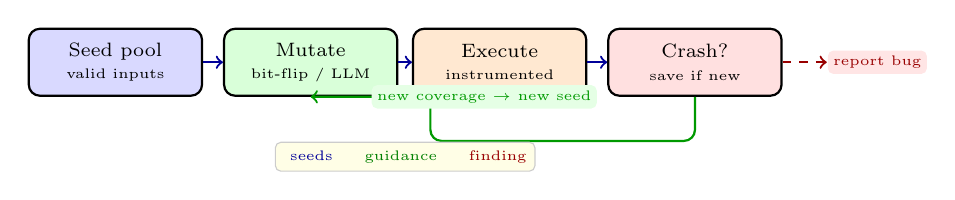
\begin{tikzpicture}[scale=0.80,every node/.style={font=\scriptsize},
  box/.style={draw,thick,rounded corners=4pt,minimum width=2.2cm,minimum height=0.85cm,align=center}]
  \node[box,fill=blue!15] (seed) at (0,0) {Seed pool\\\tiny valid inputs};
  \node[box,fill=green!15] (mut) at (3.1,0) {Mutate\\\tiny bit-flip / LLM};
  \node[box,fill=orange!18] (exec) at (6.1,0) {Execute\\\tiny instrumented};
  \node[box,fill=red!12] (crash) at (9.2,0) {Crash?\\\tiny save if new};
  \foreach \a/\b in {seed/mut,mut/exec,exec/crash}
    \draw[->,thick,blue!60!black] (\a) -- (\b);
  \draw[->,thick,green!60!black,rounded corners=4pt] (crash.south) -- ++(0,-0.7) -- ++(-4.2,0) -- ++(0,0.7) -- (mut.south) node[midway,right,font=\tiny,fill=green!10,rounded corners=2pt,inner sep=2pt] {new coverage $\to$ new seed};
  \draw[->,thick,red!60!black,dashed] (crash.east) -- ++(0.7,0) node[right,font=\tiny,fill=red!10,rounded corners=2pt,inner sep=2pt] {report bug};
  \node[font=\tiny,align=left,fill=yellow!10,draw=gray!40,rounded corners=2pt,inner sep=3pt] at (4.6,-1.5) {\textcolor{blue!60!black}{$\blacksquare$ seeds} \quad \textcolor{green!50!black}{$\blacksquare$ guidance} \quad \textcolor{red!60!black}{$\blacksquare$ finding}};
\end{tikzpicture}
\caption{Coverage-guided fuzzing loop. Seeds that discover new branches are retained; LLM guidance makes mutations more likely to be well-formed and thus reach deeper logic.}
\label{fig:fuzzing-loop}
\end{figure}

Practical fuzzing needs three ingredients: a \emph{harness} (how to call the target), a \emph{mutator} (how to change inputs), and a \emph{sanitiser} (AddressSanitizer, UBSan) that turns silent corruption into a visible crash. AI helps mainly with the mutator and harness generation.

% ============================================================
\section{The Oracle Problem and How to Sidestep It}
\label{sec:oracle-problem}
If inputs are easy and oracles are hard, the bottleneck of automated testing is not generation but \emph{judgement}. Three workarounds dominate.

\emph{Differential oracles}: run two implementations of the same spec (e.g., two regex engines) on the same input; disagreement signals a bug in at least one. \emph{Metamorphic relations}: specify how outputs should relate when inputs are transformed. For \texttt{sort}, shuffling the input should not change the output; for a compiler, adding dead code should not change the generated program. \emph{Implicit oracles}: any crash, hang, or sanitiser error is a failure even without a golden output---the basis of fuzzing.

\begin{figure}[h]\centering
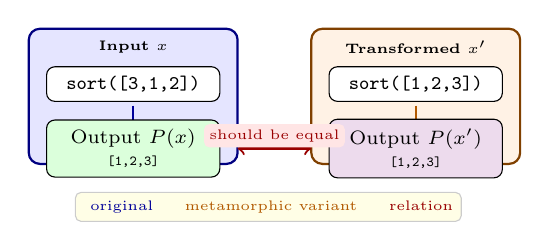
\begin{tikzpicture}[scale=0.78,every node/.style={font=\scriptsize}]
  \draw[fill=blue!10,draw=blue!50!black,thick,rounded corners=4pt] (0,0) rectangle (3.4,2.2);
  \node[font=\tiny\bfseries] at (1.7,1.9) {Input $x$};
  \node[draw,fill=white,rounded corners=3pt,minimum width=2.2cm,align=center] at (1.7,1.3) {\texttt{sort([3,1,2])}};
  \draw[->,thick,blue!60!black] (1.7,0.95) -- (1.7,0.55);
  \node[draw,fill=green!14,rounded corners=3pt,minimum width=2.2cm,align=center] at (1.7,0.25) {Output $P(x)$\\\tiny \texttt{[1,2,3]}};
  \begin{scope}[xshift=4.6cm]
    \draw[fill=orange!10,draw=orange!50!black,thick,rounded corners=4pt] (0,0) rectangle (3.4,2.2);
    \node[font=\tiny\bfseries] at (1.7,1.9) {Transformed $x'$};
    \node[draw,fill=white,rounded corners=3pt,minimum width=2.2cm,align=center] at (1.7,1.3) {\texttt{sort([1,2,3])}};
    \draw[->,thick,orange!70!black] (1.7,0.95) -- (1.7,0.55);
    \node[draw,fill=violet!14,rounded corners=3pt,minimum width=2.2cm,align=center] at (1.7,0.25) {Output $P(x')$\\\tiny \texttt{[1,2,3]}};
  \end{scope}
  \draw[<->,thick,red!60!black] (3.4,0.25) -- (4.6,0.25) node[midway,above,font=\tiny,fill=red!10,rounded corners=2pt,inner sep=2pt] {should be equal};
  \node[font=\tiny,fill=yellow!10,draw=gray!40,rounded corners=2pt,inner sep=3pt] at (3.9,-0.7) {\textcolor{blue!60!black}{$\blacksquare$ original} \quad \textcolor{orange!70!black}{$\blacksquare$ metamorphic variant} \quad \textcolor{red!60!black}{$\blacksquare$ relation}};
\end{tikzpicture}
\caption{Metamorphic oracle: shuffling the input to \texttt{sort} should not change the sorted output. The relation checks the program against itself, no golden output needed.}
\label{fig:metamorphic}
\end{figure}

\begin{example}[Metamorphic relation for median]
If $x'$ is $x$ with every element shifted by $+c$, then $\text{median}(x') = \text{median}(x)+c$. A generated test can check this relation on random $x$ and $c$ without knowing the true median in advance. Violations reveal bugs in handling of negatives or overflow.
\end{example}

No oracle is universal. The art is choosing a cheap partial oracle that catches the faults you fear most, and pairing it with a generator that explores where those faults hide.

\begin{remark}[Testing as specification]
A test suite is an executable partial specification. The oracle problem is therefore a specification problem: the more precisely you can state what ``correct'' means (as properties, relations, or a second implementation), the more you can automate checking. AI helps by inferring likely properties from code and comments, but human judgement remains the ground truth.
\end{remark}

\paragraph{Beyond crashes: non-crash oracles for fuzzing.} Modern fuzzers do not only look for crashes. They check for memory errors (sanitisers), performance regressions (timeouts), and differential discrepancies. The same loop in Fig.~\ref{fig:fuzzing-loop} applies, but the oracle box is pluggable---swap crash detection for a metamorphic check and the fuzzer searches for logic bugs instead.

% ============================================================
\section{Chapter Notes}
EvoSuite (Fraser \& Arcuri, 2011) remains the canonical search-based generator; recent LLM test-generation surveys compare it to Codex/GPT-based approaches. AFL and libFuzzer define coverage-guided fuzzing; recent work (e.g., TitanFuzz, Fuzz4All) uses LLMs as structure-aware mutators. The oracle problem is surveyed by Barr et~al.\ (2015); metamorphic testing was introduced by Chen et~al.\ (1998) and is widely used for compilers, ML systems, and databases.

% ============================================================
\section{Exercises}
\label{sec:ch03-exercises}
\begin{enumerate}[label=E3.\arabic*, leftmargin=*, itemsep=0.7em]
    \item \textbf{Coverage.} For the program in Fig.~\ref{fig:coverage}, write two tests achieving 100\% line coverage but only 50\% branch coverage, and two tests achieving 100\% branch coverage. Explain why branch coverage subsumes line coverage but not vice versa, in one sentence.
    \item \textbf{Oracle design.} For a function \texttt{reverse(s)} that reverses a string, give (a) an exact oracle, (b) a metamorphic relation, and (c) an implicit oracle. For each, state one bug it would catch and one it would miss.
    \item \textbf{Generate--filter.} You generate 100 LLM tests; 60 compile, 40 increase line coverage, and 10 of those also increase mutation score. Propose a filtering pipeline that keeps the most valuable tests first. How would you avoid keeping 40 near-duplicate tests that all cover the same new line?
    \item \textbf{Fuzzing feedback.} Explain why a blind random fuzzer struggles to reach the \texttt{else} branch of \texttt{if (x==0xdeadbeef) crash();}. How does coverage guidance help? How might an LLM mutator that has seen many hex constants help even more?
    \item \textbf{Hands-on.} Prompt any public LLM with: ``Write pytest tests for \texttt{def median(xs)} covering empty, duplicates, negatives, and large inputs.'' Run the generated tests. Report one test that has a wrong oracle (asserts the buggy behaviour) and fix it. What does this reveal about trusting generated oracles?
\end{enumerate}
% End of Chapter 3
